\documentclass{article} % For LaTeX2e
\usepackage{nips13submit_e,times}
\usepackage{hyperref}
\usepackage{epsfig}
%\usepackage{mahnig}
\usepackage{url}
\usepackage{enumerate}
\usepackage{booktabs}
%\documentstyle[nips13submit_09,times,art10]{article} % For LaTeX 2.09
\usepackage{multicol}


\title{Simulating the Izhikevich spiking neuron model using
the Brian2 software}

\author{Julen Etxaniz and Ibon Urbina}

% The \author macro works with any number of authors. There are two commands
% used to separate the names and addresses of multiple authors: \And and \AND.
%
% Using \And between authors leaves it to \LaTeX{} to determine where to break
% the lines. Using \AND forces a linebreak at that point. So, if \LaTeX{}
% puts 3 of 4 authors names on the first line, and the last on the second
% line, try using \AND instead of \And before the third author name.

\newcommand{\fix}{\marginpar{FIX}}
\newcommand{\new}{\marginpar{NEW}}

\nipsfinalcopy % Uncomment for camera-ready version

\begin{document}

\maketitle

\begin{abstract}
In this document we report our proposal for the Izhikevich spiking neuron model representation in Brian2 Python's library, which is a simulator for spiking neural networks. We manage to successfully implement most of the proposed neuron types and features. We also make a simulation with a network of 1000 neurons. The original code was proposed by the author in the MATLAB programming language, but taking into account the importance Python programming language is taking in Machine Learning task implementations, we believe that it is convenient to also have an implementation with Python.
\end{abstract}

\tableofcontents

\section{Description of the problem}

% Copied from project description. Change the text

The study of spike-timing dynamics in the brain is of interest to neuroscientists and the artificial network community. Investigation of the relative timing of spikes of multiple neurons \cite{Izhikevich2008LargescaleMO} and the role they play in temporal coding in the brain is an important issue. Similarly, spiking networks can serve as powerful supervised learning and memory representation tools with several potential applications in the machine learning domain \cite{PaugamMoisy2008DelayLA}.

The Izhikevich spiking neuron model \cite{Izhikevich2003Simple} \cite{Izhikevich2004Which} is a two-dimensional system of ordinary differential equations. In the equations shown in Figure \ref{fig:model}, variable \(v\) represents the membrane potential of the neuron and \(u\) represents a membrane recovery variable, which accounts for the activation of \(K^+\) ionic currents and the inactivation of Na ionic currents, and provides negative feedback to \(v\).

\begin{figure}[ht]
    \centering
    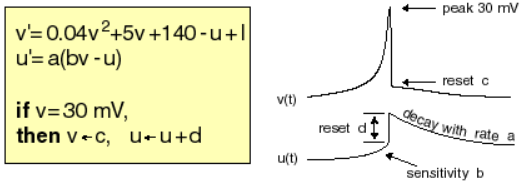
\includegraphics{model.png}
    \caption{Izhikevich’s spiking neuron model. Electronic version of the figure and reproduction permissions are freely available at \url{www.izhikevich.com}}
    \label{fig:model}
\end{figure}

The goal of the project is to implement the Izhikevich’s model using the Brian2 Python library \url{https://brian2.readthedocs.io/en/stable/}. Then, test that for different parameters of the model it is possible to reproduce the spiking patterns described in \cite{Izhikevich2003Simple} \cite{Izhikevich2004Which}.

\section{Understanding the Izhikevich spiking neuron model}

\subsection{A new paradigm}
The fact that recent physiological experiments demonstrate that neural code and thus, neural information, is founded on the time of individual action potentials (individual spikes) changes the governing paradigm over the last years regarding to neural encoding: neural information is encoded in the firing rate of neurons.

This new paradigm does not exclude the previous one, but yes, give us a new perspective. Moreover, it has carried out a new class of neural models called Spiking Neural Networks (SNN).

Due to the fact that these type of networks reproduce our biological neurons better than other artificial neural networks (ANN), not only do they provide powerful tools for analysis of elementary processes in the brain, but also are able to process substantial amount of data using relatively small number of spikes. Furthermore, it has been scientifically demonstrated that they are capable of resolving all problems solved by non-spiking neural networks plus the ones that those are not capable of. 

\subsection{Biological neurons}
The neuron is the basic building block of the brain and central nervous system. Moreover, they are specialized cells that transmit chemical and electrical signals. Thus, in essence, they are cells with common cell components (such as nucleus, organelles, cytoplasm, mitochondria, etc); but, with exclusive structures for receiving and sending the electrical signals that make neuronal communication possible. Which are these special structures? The most important ones, behind:
\begin{itemize}
    \item \textbf{Dendrite}:
    branch-like structures extending away from the cell body that receive messages from other neurons and allow them to travel to the cell body.
   
    \item \textbf{Axon}:
    tube-like structure that carries an electrical impulse from the cell body to the opposite end of the neuron, the axon terminals, which pass the impulse to another neuron.
    
    \item \textbf{Synapse}:
    chemical junction between the axon terminals of one neuron and the dendrites of the next.
\end{itemize}

As common cells, neurons are surrounded by a cell membrane which completely separates the cell from its external environment. In neurons, this is the membrane that allows positive or negative ions to flow into and out of it. The inside of the cell is usually more negative than the outside; scientific studies talk about a negative difference of 70 \(mv\) with respect to the outside. This difference is known as the membrane potential, so, it defines the difference in electric potential between the interior and the exterior of the neuron. This term is not a static variable and changes constantly depending on the inputs coming from the axons of other neurons or from the exterior: some inputs make the membrane potential being more positive (less negative) or less positive (more negative).

But, how do biological neurons communicate with each other? 

As we mentioned above, depending on the input a neuron receives, its membrane potential can be modified. This occurs because when an action potential reaches the presynaptic terminal, that are the axon terminals of the neuron, different neurotransmitters (chemicals) are released to the postsynaptic dendrite. Depending on what chemical is released, positive or negative ions will be attached to the membrane potential, and therefore, the potential will be modified. When the membrane potential reaches a potential value called action potential threshold, an action potential (or spike) is released; sometimes it is said that a neuron has fired a spike.

Let's resume the communication process:
\begin{itemize}
    \item An electrical input reaches the presynaptic neuron.
    
    \item The electrical signal is converted into a chemical signal in the form of neurotransmitter release.
    
    \item Postsynaptic neuron receptors catch the chemicals released by the presynaptic neuron.
    
    \item Postsynaptic neuron membrane potential is modified due to the ion flow of the received neurotransmitters.
\end{itemize}

No matter what type of signal is transmitted (chemical or electric) but both need a stimuli (electrical activity) in the presynaptic neuron. This stimuli is usually given in two ways: by an external current input (in scientific experiments for example) or as a consequence of another presynaptic current induction. 

To finish with this brief explanation of how biological neurons are and behave and to understand future concepts, it is convenient to introduce what excitatory and inhibitory neurotransmitters are. For now, lets refer to neurotransmitters as the body's chemical messengers. As mentioned before, they are the molecules used by the nervous system to transmit messages between neurons, or from neurons to muscles. A neurotransmitter can  influence a neuron in two ways:
\begin{itemize}
    \item \textbf{Excitatory}: a neurotransmitter that promotes the generation of the electrical signal (action potential) in the receiving neuron.
   
    \item \textbf{Inhibitory}: a neurotransmitter that prevents the generation of the electrical signal (action potential) in the receiving neuron.
    
\end{itemize}

\subsection{Biological neurons and spiking models}
3 properties are shared in both biological and spiking models:
\begin{itemize}
    \item \textbf{Output signals}:
    The coming information is delivered via many inputs, but a single spiking signal is produced as an output.
    
    \item \textbf{Firing}:
    The probability of generating a spike is increased by excitatory inputs and decreased by inhibitory inputs. 
    
    \item \textbf{Dynamic}:
    The spiking flow or spiking generation is characterized by at least one state variable. When the internal variables of the model reach a certain state (a certain threshold), the model generates one or more spikes (a burst of spikes).
\end{itemize}

\subsection{Why Izhikevich spiking neuron model?}
Neuroscience, the scientific study of the nervous system which goal is to understand the fundamental and emergent properties of neurons and neural circuits, not only requires experimental studies with animals and humans, but also models that are able to simulate with numerical means a large-scale of brain models.

However, until the emergence of the Izhikevich model, it was not easy to find an adequate balance between good biological neurons representation and a low computational cost. For instance, coexisted models with very rich biological representation but computationally prohibitive (Hodgkin-Huxley-type model) and simple and unrealistic biological neuron characterization but computationally exceptional. 

Two were the requirements demanded to artificial brain models:
\begin{itemize}
    \item Computationally simple.
    
    \item Capable of producing rich firing patterns exhibited by real biological neurons.
\end{itemize}
 
That's why the arrival of the Izhikevich model has been a fascinating improvement in this field. Apart from being biologically as plausible as the Hodgkin-Huxley model, it is also as computationally efficient as the integrate-and-fire model. For instance, changing four parameters of the model, one can reproduce the spiking and bursting dynamics of known types of cortical neurons.

\subsection{Cortical neurons}
Cortical neurons correspond to the ones living in the cerebral cortex; which is the outer layer of the neural tissue of the brain in humans and other mammals. This cortex is the largest site of neural integration in the central nervous system and plays a key role in attention, perception, awareness, thought, memory, language and consciousness.

The cerebrum, the largest part of the brain containing the cerebral cortex and the uppermost region of the central nervous system, is the most highly developed part of the human brain and is responsible for thinking, perceiving, producing and understanding language. Moreover, it is directly or indirectly involved in several functions of the body, such as determining intelligence, determining personality, motor functions, planning and organization, touch sensation, processing sensory information, language processing...

As we may notice, most information processing occurs in the cerebral cortex. Thus, we may make an idea of the importance of analyzing and representing the cortical neurons in an artificial way in order to reproduce human processing and learning. As mentioned before, it is exactly the type of neurons the Izhikevich model can  simulate. Furthermore, it can also simulate neural features and behaviours mentioned in the next section.

\subsection{Neuro-computational features and information processing}
Neurons are not limited to a single spike or action potential; they may release more than one and with different patterns depending on two variables: time and input current. Analyzing this firing-behaviour has an utmost importance regarding to the new paradigm: spike-timing information processing.

Below, 20 of the most prominent features of biological spiking neurons mentioned in \cite{Izhikevich2004Which}. See Figure \ref{fig:features}.

\begin{figure}[ht]
    \centering
    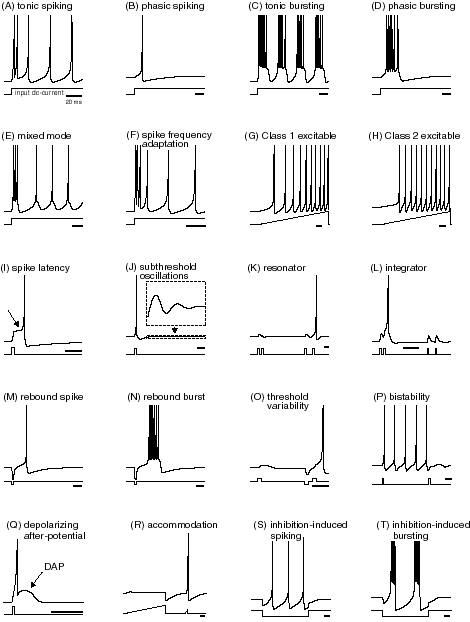
\includegraphics[width=\linewidth]{features.png}
    \caption{Electronic version of the figure and reproduction permissions are freely available at \url{www.izhikevich.com}}
    \label{fig:features}
\end{figure}

\begin{itemize}
    \item \textbf{Tonic Spiking}:
    \begin{itemize}
        \item Neurons are quiescent (inactive) until they are stimulated.
        \item When the input is on, the neuron continue to fire a train of spikes.
        \item Information processing: can indicate that there is a persistent input.
    \end{itemize}
    
    \item \textbf{Phasic Spiking}:
    \begin{itemize}
        \item Neurons fire a single spike at the onset of the input and remain quiescent afterwards.
        \item Information processing: can detect the beginning of the stimulation.
    \end{itemize}
    
    \item \textbf{Tonic Bursting}:
    \begin{itemize}
        \item Neurons fire periodic bursts of spikes when stimulated.
        \item Contribute to the gamma-frequency oscillations in the brain.
    \end{itemize}
    
    \item \textbf{Phasic Bursting}:
    \begin{itemize}
        \item Neurons fire phasic bursts of spikes at the onset of the input.
        \item Information processing: can report the beginning of the stimulation.
        \item Information processing: can recognized the channel of communication between neurons because the interspike frequency within the bursts encodes that channel. 
    \end{itemize}
    
    \item \textbf{Mixed Model (Bursting Then Spiking)}:
    \begin{itemize}
        \item Neurons fire a phasic burst at the onset of the stimulation and then switch to the tonic spiking mode.
        \item Information processing: can detect the onset and report the extent of the stimulation.
    \end{itemize}
    
    \item \textbf{Spike Frequency Adaptation}:
    \begin{itemize}
        \item Neurons fire tonic spikes with decreasing frequency.
        \item The frequency is relatively high at the onset of stimulation, and then it adapts.
        \item Information processing: can encode the time elapsed since the onset of the input thanks to the interspike frequency.
    \end{itemize}
    
    \item \textbf{Class 1 Excitatory}:
    \begin{itemize}
        \item The frequency of tonic spiking depends on the strength of the input.
        \item Neurons fire low-frequency spikes when the input is weak.
        \item Information processing: can encode the strength of the input.
    \end{itemize}
    
    \item \textbf{Class 2 Excitability}:
    \begin{itemize}
        \item Neurons are either quiescent or fire a train of spikes with a certain relatively large frequency.
        \item Cannot fire low-frequency spike trains.
        \item Their firing rate is a poor predictor of the strength of stimulation.
    \end{itemize}
    
    \item \textbf{Spike Latency}:
    \begin{itemize}
        \item Neurons fire spikes with a delay that depends on the strength of the input signal.
        \item For weak but high-threshold input, the delay (spike latency) can be quite large.
        \item Information processing: can encode the strength of the input thanks to the latencies.
    \end{itemize}
    
    \item \textbf{Subthreshold Oscillations}:
    \begin{itemize}
        \item Neurons capable of exhibiting oscillatory potentials.
        \item Oscillations frequencies play an important role and act as bandpass filters.
    \end{itemize}
    
    \item \textbf{Frequency Preference and Resonance}:
    \begin{itemize}
        \item Neurons having oscillatory potentials can respond selectively to the inputs having frequency content similar to the frequency of subthreshold oscillations.
    \end{itemize}
    
    \item \textbf{Integration and Coincidence Detection}:
    \begin{itemize}
        \item Neurons without oscillatory potentials.
        \item The higher the frequency of the input, the more likely they fire.
        \item Information processing: can be useful for detecting coincident or nearly coincident spikes.
    \end{itemize}
    
    \item \textbf{Rebound Spike}:
    \begin{itemize}
        \item When a neuron receives and then is released from an inhibitory input, it may fire a post-inhibitory spike.
    \end{itemize}
    
    \item \textbf{Rebound Burst}:
    \begin{itemize}
        \item When a neuron receives and then is released from an inhibitory input, it may fire post-inhibitory bursts.
    \end{itemize}
    
    \item \textbf{Threshold Variability}:
    \begin{itemize}
        \item Depending on the prior activity of the neurons, biological neurons have a variable threshold.
    \end{itemize}
    
    \item \textbf{Bistability of Resting and Spiking States}:
    \begin{itemize}
        \item Neurons that exhibit two stable modes of operation: resting and tonic or bursting spiking.
        \item To switch from the tonic spiking to resting mode, the input must arrive at an appropriate phase of the oscillation.
        \item Information processing: can create a short-term memory.
    \end{itemize}
    
    \item \textbf{Depolarizing After-Potentials}:
    \begin{itemize}
        \item After firing a spike, the membrane potential of a neuron may exhibit a prolonged after-hyperpolarization or a prolonged depolarized after-potential.
    \end{itemize}
    
    \item \textbf{Accommodation}:
    \begin{itemize}
        \item Neurons are extremely sensitive to brief coincident inputs, but may not fire in response to a strong but slowly increasing input.
    \end{itemize}
    
    \item \textbf{Inhibition-Induced Spiking}:
    \begin{itemize} 
        \item Neurons are quiescent (inactive) when there is no input, but fire when hyperpolarized by an inhibitory input or an injected current.
    \end{itemize}
    
    \item \textbf{Inhibition-Induced Bursting}:
    \begin{itemize}
        \item Neurons fire tonic bursts of spikes in response to a prolonged hyperpolarization.
        \item It is believed that this burstings plays an important role in sleep rhythms.
    \end{itemize}
    
\end{itemize}


\subsection{Neuron Types}

Before we start analyzing and understanding the long-awaited Izkhivevich model, it is convenient to have a subtle idea of the different cortical neurons we can encounter with according to \cite{Izhikevich2003Simple}. See Figure \ref{fig:types}.

\begin{figure}[ht]
    \centering
    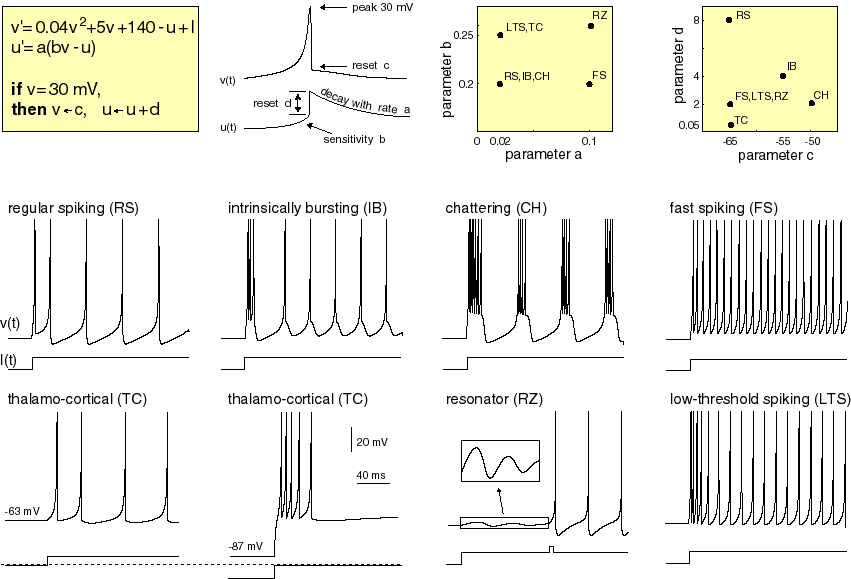
\includegraphics[width=\linewidth]{types.png}
    \caption{Neuron Types. Electronic version of the figure and reproduction permissions are freely available at \url{www.izhikevich.com}}
    \label{fig:types}
\end{figure}

In the case of the neocortical neurons in the mammalian brain, depending on the pattern of spiking and bursting, excitatory cells are divided into three classes:

\begin{itemize}
    \item \textbf{Regular spiking (RS)}:
    \begin{itemize}
        \item The most typical neurons in the cortex.
        \item When a prolonged stimulus is injected, the neurons fire a few spikes with short interspike period and then the period increases.
    \end{itemize}
    
    \item \textbf{Intrinsically bursting (IB)}:
    \begin{itemize}
        \item Fire a stereotypical burst of spikes followed by repetitive single spikes.
    \end{itemize}
    
    \item \textbf{Chattering (CH)}:
    \begin{itemize}
        \item The stereotypical bursts of closely spaced spikes.
    \end{itemize}
    
\end{itemize}

In addition, depending also on spiking and bursting patterns, inhibitory cells are divided in two classes:

\begin{itemize}
    \item \textbf{Fast spiking (FS)}:
    \begin{itemize}
        \item Fire periodic trains of action potentials with extremely high frequency practically without any adaptation; that is, without practically a slowing down in the frequency.
    \end{itemize}
     
    
    \item \textbf{Low-threshold spiking (LTS)}:
     \begin{itemize}
        \item Fire periodic trains of action potentials with extremely high frequency with noticeable spike frequency adaptation; that is, with a noticeable slowing down in the frequency.
    \end{itemize}
\end{itemize}

However, this model is not only limited to representing cerebral cortex neurons. For instance, it can reproduce thalamo-cortical cells; those that convey sensory information to the neocortex via thalamo-cortical synapses. We have to take into account that the thalamus is the door which introduces cells to the neocortex. Such is the importance of the thalamus, that every single sensory information except the olfactive one is processed in the neocortex thanks to it. How that sensory information reaches the thalamus is out of the scope.

Two are the possible dynamics of the thalamo-cortical cells depending on the firing regimes:

\begin{itemize}
    \item \textbf{At rest \(v\) is around \(-60mV\) and then depolarized}:
     \begin{itemize}
        \item They exhibit tonic firing; which refers to a sustained response that activates during the course of the stimulus.
    \end{itemize}
    
    \item \textbf{A negative current step is delivered and the membrane potential is hyperpolarized}:
     \begin{itemize}
        \item Neurons fire a rebound burst of action potentials.
    \end{itemize}
\end{itemize}

Finally, to finish with the dynamics the model can represent, there is another neuron behaviour called resonator that is convenient to mention. Apart from this one, others with minor importance in the research can be represented either: brainstem, hyppocampus, basal ganglia and olfactory bulb.

\begin{itemize}
    \item \textbf{Resonator (RZ) }:
     \begin{itemize}
        \item Neurons have damped or sustained subthreshold oscillations. 
        \item They resonate to rhythmic inputs having appropriate frequency.
    \end{itemize}
\end{itemize}

\subsection{The Izhikevich model}

In the Izhikevich model proposed in \cite{Izhikevich2003Simple}, the author reduced the model to a two-dimensional system of ordinary differential equations plus an auxiliary after-spike resetting behaviour. The model can exhibit firing patterns of cortical neurons with the choice of parameters \(a\), \(b\), \(c\) and \(d\), taking only 13 floating point operations to simulate 1 \(ms\) of the model (at least in MATLAB).

The author recalls that the \(+30mV\) is not a threshold, but the peak of the spike. The real value of the threshold is between \(-70\) and \(-50\); being a dynamic value as in biological neurons.

\begin{itemize}
    \item \textbf{The differential equations}:
            \begin{itemize}
                 \item \( \frac{dv}{dt} = 0.04v^2 + 5v + 140 - u + I \) 
                 \item \( \frac{dv}{dt} = a(bv - u) \)
            \end{itemize}
    \item \textbf{The after-spike resetting function}:
            \begin{itemize} 
            \item
            \(if \hspace{1 mm} v \geq 30mV,  \hspace{1 mm} then 
            \left \{ \begin{array}{lcc}
                      v \leftarrow c \\
                      \\ u \leftarrow u+d \\
                       \end{array}
             \right. \)
             \end{itemize}
\end{itemize}

Where, 
\begin{itemize}
    \item \textbf{Dimensionless variables}:
     \begin{itemize}
        \item \(v\), the membrane potential of the neuron.
        \item \(u\), the membrane recovery variable, which accounts for the activation of \(K^+\) ionic currents and inactivation of \(Na^+\) ionic currents. Thus, it provides a negative feedback to v.
    \end{itemize}
    \item \textbf{Dimensionless parameters}:
     \begin{itemize}
        \item \(a\), the time scale of the recovery variable \(u\). 
        \item \(b\), the sensitivity of the recovery variable \(u\) to the subthreshold fluctuations of the membrane potential \(v\).
        \item \(c\), the after-spike reset value of the membrane potential \(v\) caused by the fast high-threshold \(K^+\) conductances.
        \item \(d\), the after-spike reset of the recovery variable \(u\) caused by slow high-threshold \(Na^+\) and \(K^+\).
        \item \(t\), the time.
     \end{itemize}
     \item \textbf{Scale}:
      \begin{itemize}
        \item \(v\) has \(mV\) scale.
        \item \(t\), has \(ms\) scale.
     \end{itemize}
     
\end{itemize}

\section{Implementation}

Firstly, we completed Jupyter Notebooks from Brian2 tutorial available at \url{https://brian2.readthedocs.io/en/stable/resources/tutorials}. They helped us understand how SNNs and Brian2 work. Then we read the 2 papers \cite{Izhikevich2003Simple} \cite{Izhikevich2004Which} that describe the Izhikevich model. Finally, we implemented the model and simulated the proposed neuron types, features and simulation. To help with the implementation we used resources available at \url{https://www.izhikevich.org/publications/spikes.htm} and \url{https://www.izhikevich.org/publications/whichmod.htm}. For example, the MATLAB code was very helpful.

All the project steps were implemented in a Jupyter Notebook with Python. All the resulting images can be visualized there. We mainly used \texttt{Brian2} library. We also used \texttt{ipywidgets} for interaction and \texttt{matplotlib} for visualization. The project description, the written report, the notebooks and relevant papers are available at \url{https://github.com/juletx/spiking-neural-network}.

We organized the implementation of the project according to the following tasks.

\subsection{Importing the libraries}
We mainly used \texttt{Brian2} library. We also used \texttt{ipywidgets} for interaction and \texttt{matplotlib} for visualization.

\subsection{Defining the model}
We defined the model as a python function that receives the parameters of the model as input. Fistly, we define the neuron with the equations. Then, we create a monitor to measure the values of the neron. Next, we run the simulation for the specified duration. Finally plot the result uding matplotlib. 

We tried to make it flexible enough to adjust to all the neuron types and features. As we advanced through neuron types and features we had to make some adjustments to increase flexibility. For example, we decided to pass I as a function instead of a fixed value. Some simulations required changing I and this avoids having to copy the model at those. However, there were some cases that it wasn't possible because bigger changes had to be done. For instance, Class 1 Excitable required changing the differential equation for v. In those cases we copied the model and changed the necessary parts.

\subsection{Interacting with the model}
We used \texttt{ipywidgets} to create sliders that allow interacting with the model by changing the parameters. By playing a bit with the sliders it is clear that the types of spikes are very diverse. In the next sections we define and simulate those types.
 
\subsection{Neuron Types}
We defined the neuron types using the parameters from \cite{Izhikevich2003Simple}. The duration wasn't specified so we chose duration that was reasonable for all the types. That way, we didn't have to specify the duration and fI function for each neuron type. We decided to change the time step from 0.1 to 0.25 so that the simulation was faster. Otherwise, the duration had to be quite long to see enough spikes.

\subsection{Neuron Features}
We defined the neuron features using the parameters from \url{https://www.izhikevich.org/publications/whichmod.htm}. In most of the cases the default parameters weren't working as expected. We realised that sometimes increasing the times was enough. In most of the cases after some tries we achieved a good result. However, there were some cases where we couldn't find the correct parameters.

\subsection{Defining the simulation}
We define the simulation that is proposed in \cite{Izhikevich2003Simple} and implemented in \url{https://www.izhikevich.org/publications/spikes.htm}. See Figure \ref{fig:simulation} for an illustration of the simulation. This simulation creates a network of 1000 neurons, 800 excitatory and 200 inhibitory. The simulation is run for 1000 ms. It doesn't use any of the previously mentioned types. Instead, some values are calculated randomly to add some variability similar to biological neurons. Moreover, we decided to do something similar to the model to allow some flexibility. We added the number of neurons, time step and duration as parameters.

First, we define the equations and excitatory and inhibitory neuron groups. Next, we define the synapses between neurons, connecting all the neurons with random weights. Then, we create the monitor to record the values and run the simulation. Finally, we plot the a graph with the times of all the spikes and another one with the values of the first neuron.

\begin{figure}[ht]
    \centering
    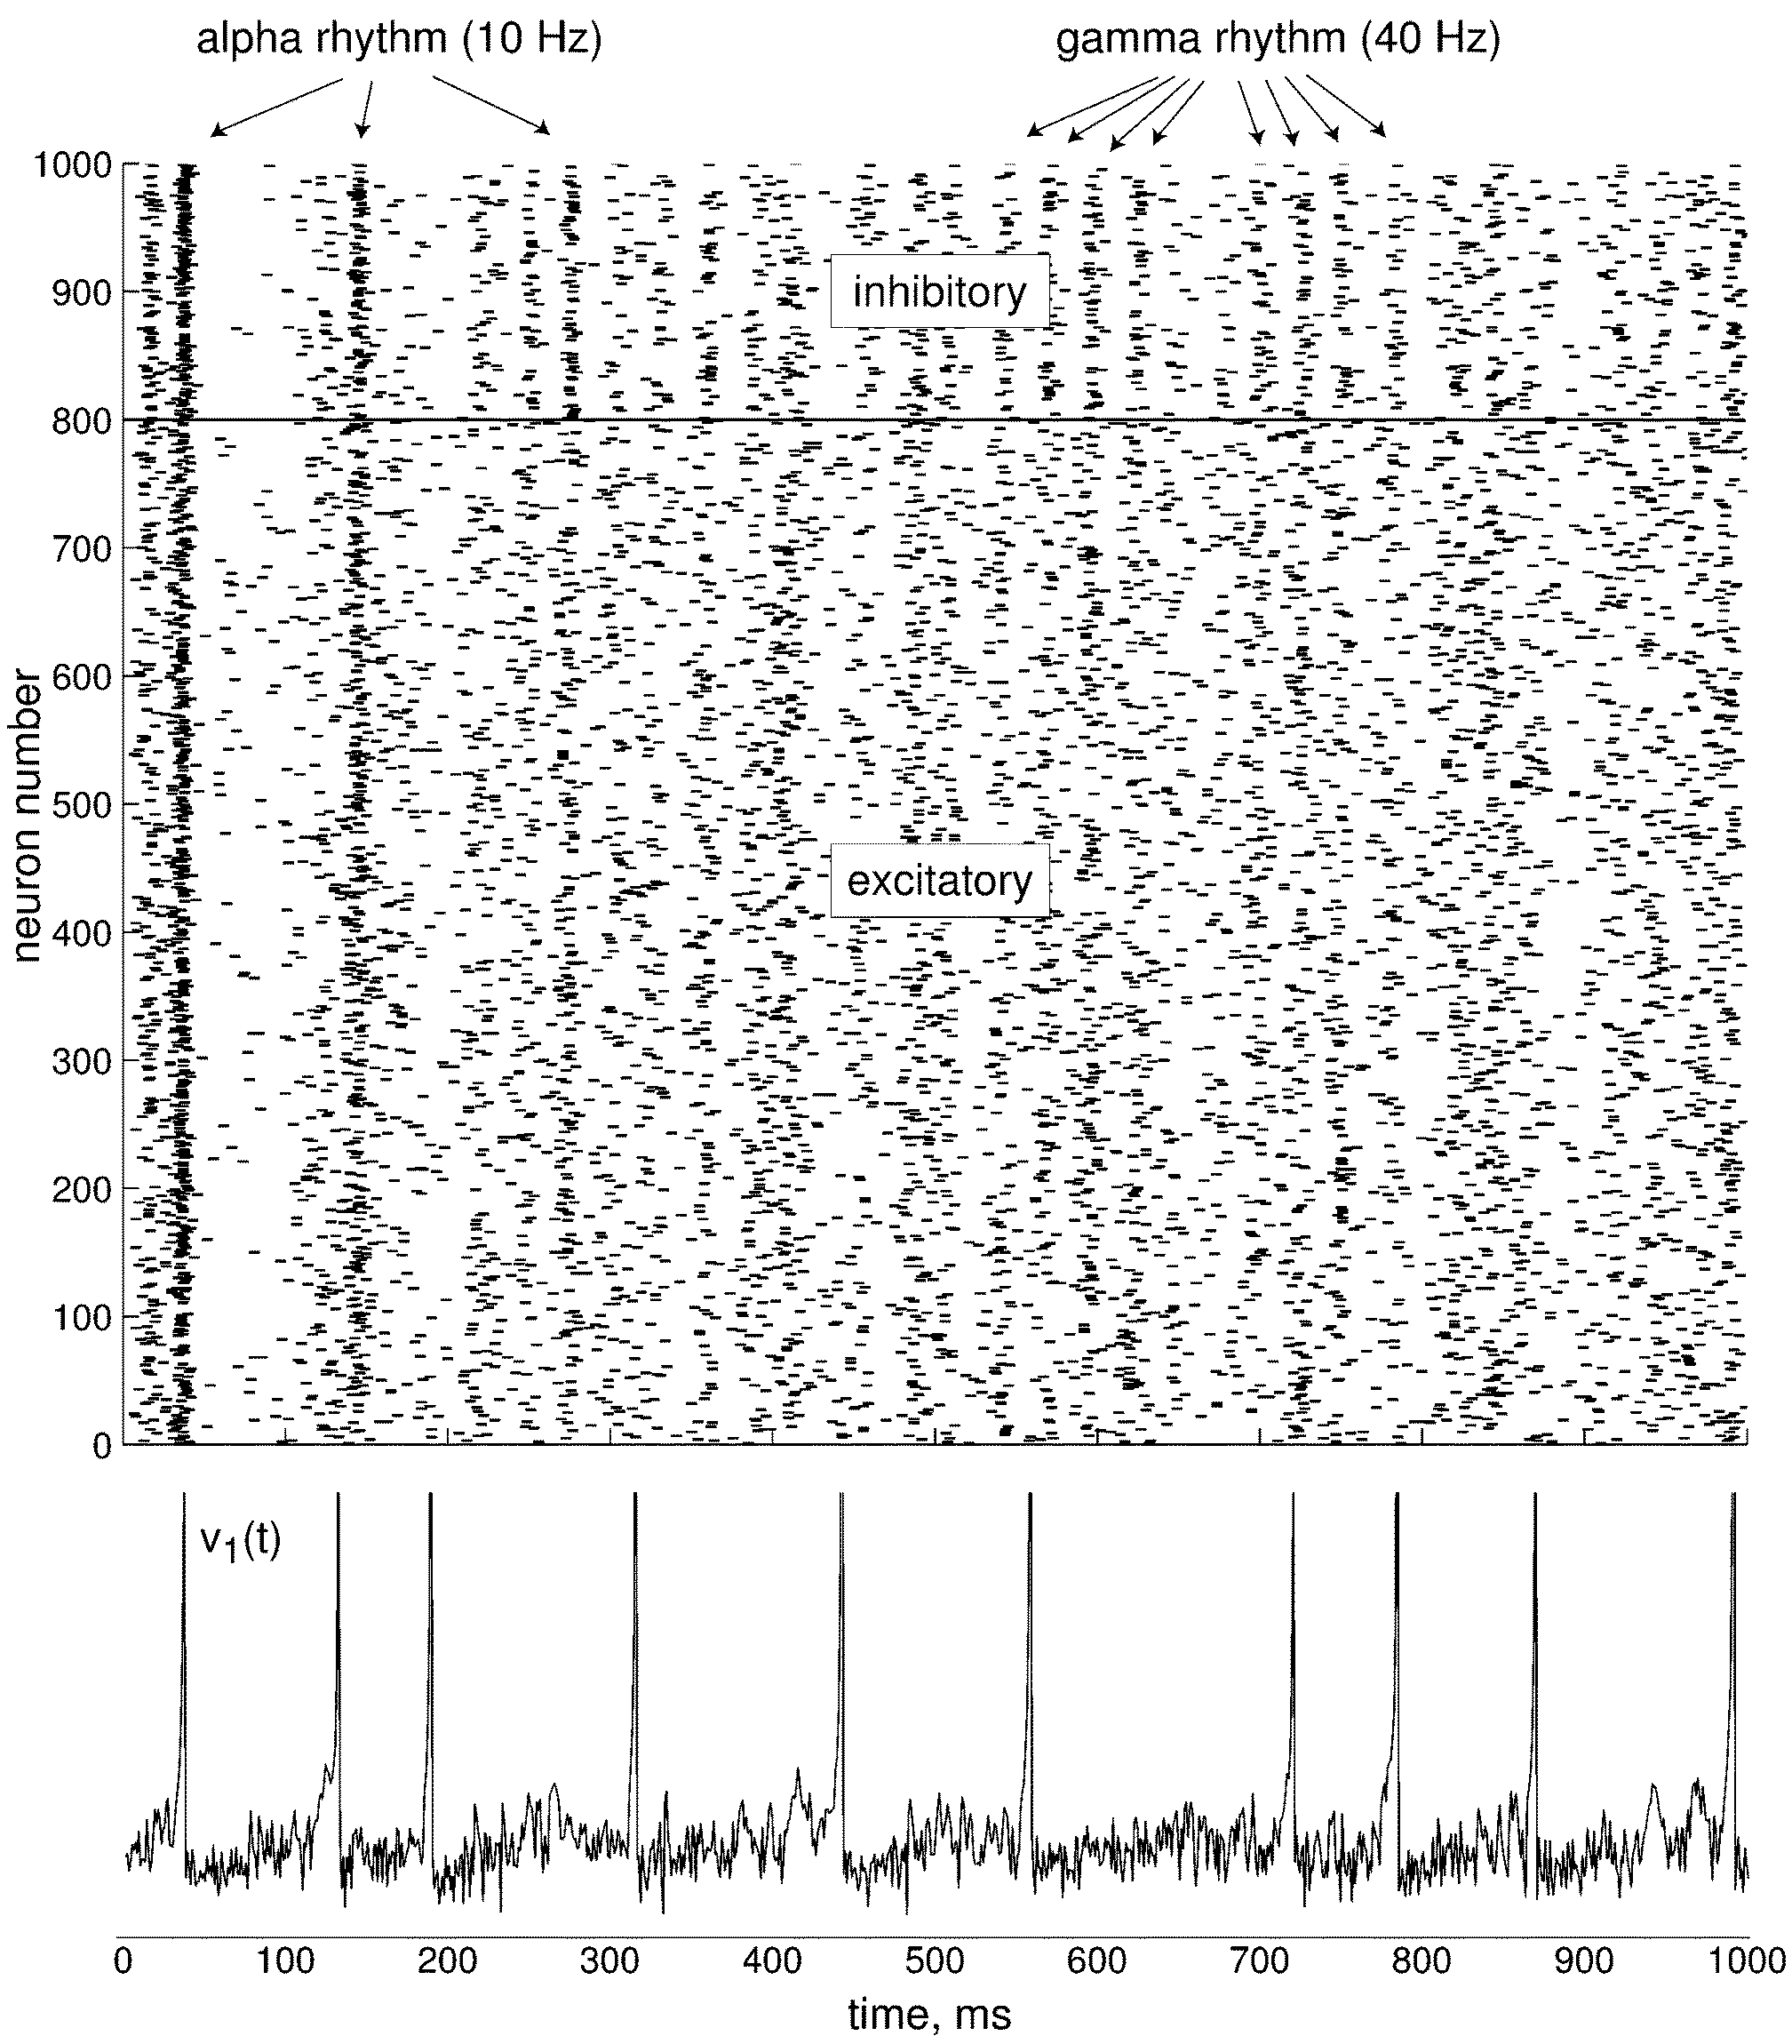
\includegraphics[width=\linewidth]{simulation.png}
    \caption{Simulation of a network of 1000 neurons. At the top we can see all the spikes of the neurons though time. At the bottom, we can see the behaviour of one of those neurons.}
    \label{fig:simulation}
\end{figure}

\subsection{Running the simulation}
We used \texttt{ipywidgets} to create sliders that allow interacting with the model by changing the parameters. The number of neurons can be increased up to 10000. The number of excitatory and inhibitory neurons can be changed separately to allow different rates than 4 to 1. The time resolution and duration can also be adjusted.

\section{Results}

\subsection{Neuron Types}
We managed to simulate all the types mentioned in \cite{Izhikevich2003Simple} correctly except for the Resonator. We tried changing the parameters but we couldn't find the correct combination. We decided to change the time step from 0.1 to 0.25 so that the simulation was faster. The duration of each simulation wasn't specified so we chose 1000 ms so that it was long enough for all the types. Figures of all the neuron types can be seen at the Jupyter Notebook.

\subsection{Neuron Features}
We achieved a correct result in most of the features that are introduced in \cite{Izhikevich2004Which} by making some adjustments. We have also included the simulations with the proposed parameters so that they can be compared with ours. In general, increasing the duration and the times in the I function was enough. In some cases other adjustments had to be done with different parameters. And there were also some features where we didn't achieve the expected result even if we tried many combinations. Figures of all the neuron features can be seen at the Jupyter Notebook.

\subsection{Simulation}
The result obtained with the same parameters is a bit different to \cite{Izhikevich2003Simple}. However, similar rhythmic behaviour can be achieved by changing the parameters. This can be obtained by increasing the number of neurons and/or increasing tau. For instance, combining 2500 excitatory and 1000 inhibitory neurons with the default tau produces short rhythmic behaviour. The simulation can be run in the Jupyter Notebook to obtain the figures.

\section{Conclusions}
The Izhikevich model is a powerful model that can simulate many neuron types and features. We haven't managed to simulate all the behaviours, but we achieved most of them. It is also notable that it is computationally efficient and therefore the simulations take few seconds. Even when simulating with a big network of neurons the needed time is reasonable.

We have experimented with Brian2 library and we think that it is a great tool for simulating Spiking Neural Networks. It makes defining the models, simulating and visualization much easier. However, we have clearly seen that replicating the results proposed at \cite{Izhikevich2003Simple} \cite{Izhikevich2004Which} isn't that easy. In most of the cases some parameters had to be changed, and there were some cases where we didn't find the correct parameters. This is a common problem with simulations, replicating the results can be challenging even when the code is the same. When we take into account that we were using a different language and library, it isn't surprising that we had some difficulties.

\bibliographystyle{unsrt}
\bibliography{bibtex_references_project}

\end{document}
